\scanpage{31}
\margin{\figure{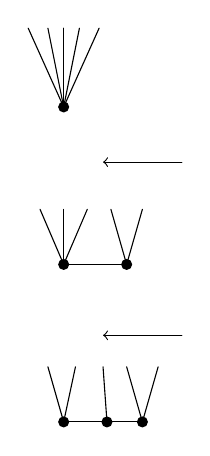
\begin{tikzpicture}[x=1cm,y=1cm,line cap=round,line join=round]\fill (0,4) circle(2pt);\foreach \x in {-.45,-.2,0,.2,.45}{\draw (0,4)--(\x,5);}\draw (0,2)--(.8,2);\fill (0,2) circle(2pt);\fill (.8,2) circle(2pt);\foreach \x in {-.3,0,.3}{\draw (0,2)--(\x,2.7);}\draw (.8,2)--(.6,2.7);\draw (.8,2)--(1,2.7);\draw (0,0)--(.55,0)--(1,0);\foreach \x in {0,.55,1}{\fill (\x,0) circle(2pt);}\draw (0,0)--(-.2,.7);\draw (0,0)--(.15,.7);\draw (.55,0)--(.5,.7);\draw (1,0)--(.8,.7);\draw (1,0)--(1.2,.7);\draw[->] (1.5,3.3)--(.5,3.3);\draw[->] (1.5,1.1)--(.5,1.1);\end{tikzpicture}}}

\sbox{180}{\figure{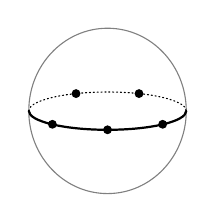
\begin{tikzpicture}[x=1cm,y=1cm,line cap=round,line join=round]\draw[gray] (0,0) ellipse (1 and 1.05);\draw[thick] (-1,0) arc[start angle=180,end angle=360,x radius=1,y radius=.24];\draw[densely dotted] (-1,0) arc[start angle=180,end angle=0,x radius=1,y radius=.24];\fill (-0.7,-0.17) circle(1.6pt);\fill (0,-0.24) circle(1.6pt);\fill (0.7,-0.17) circle(1.6pt);\fill (-0.4,0.22) circle(1.6pt);\fill (0.4,0.22) circle(1.6pt);\end{tikzpicture}}}
\sbox{181}{\figure{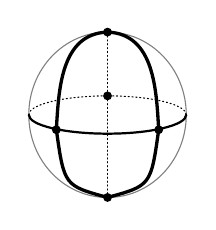
\begin{tikzpicture}[x=1cm,y=1cm,line cap=round,line join=round]\draw[gray] (0,0) ellipse (1 and 1.05);\draw[thick] (-1,0) arc[start angle=180,end angle=360,x radius=1,y radius=.24];\draw[densely dotted] (-1,0) arc[start angle=180,end angle=0,x radius=1,y radius=.24];\draw[very thick] (0,1.05) .. controls (-.6,1.03) and (-.62,.3) .. (-.65,-.19);\draw[very thick] (0,1.05) .. controls (.6,1.03) and (.62,.3) .. (.65,-.19);\draw[densely dotted] (0,1.05)--(0,.24);\draw[very thick] (-.65,-.19) .. controls (-.55,-.9) .. (0,-1.05) .. controls (.55,-.9) .. (.65,-.19);\draw[densely dotted] (0,.24)--(0,-1.05);\fill (0,1.05) circle(1.6pt);\fill (-0.65,-0.19) circle(1.6pt);\fill (0.65,-0.19) circle(1.6pt);\fill (0,0.24) circle(1.6pt);\fill (0,-1.05) circle(1.6pt);\end{tikzpicture}}}
\sbox{182}{\figure{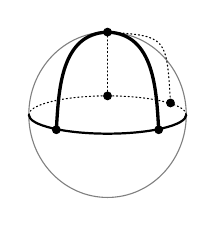
\begin{tikzpicture}[x=1cm,y=1cm,line cap=round,line join=round]\draw[gray] (0,0) ellipse (1 and 1.05);\draw[thick] (-1,0) arc[start angle=180,end angle=360,x radius=1,y radius=.24];\draw[densely dotted] (-1,0) arc[start angle=180,end angle=0,x radius=1,y radius=.24];\draw[very thick] (0,1.05) .. controls (-.6,1.03) and (-.62,.3) .. (-.65,-.19);\draw[very thick] (0,1.05) .. controls (.6,1.03) and (.62,.3) .. (.65,-.19);\draw[densely dotted] (0,1.05)--(0,.24);\draw[densely dotted] (0,1.05) .. controls (.75,1) .. (.8,.15);\fill (0,1.05) circle(1.6pt);\fill (-0.65,-0.19) circle(1.6pt);\fill (0.65,-0.19) circle(1.6pt);\fill (0,0.24) circle(1.6pt);\fill (0.8,0.15) circle(1.6pt);\end{tikzpicture}}}
\sbox{183}{\figure{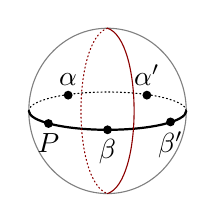
\begin{tikzpicture}[x=1cm,y=1cm,line cap=round,line join=round]\draw[gray] (0,0) ellipse (1 and 1.05);\draw[thick] (-1,0) arc[start angle=180,end angle=360,x radius=1,y radius=.24];\draw[densely dotted] (-1,0) arc[start angle=180,end angle=0,x radius=1,y radius=.24];\draw[red!55!black] (0,1.05) .. controls (.45,.9) and (.45,-.9) .. (0,-1.05);\draw[red!55!black,densely dotted] (0,1.05) .. controls (-.45,.9) and (-.45,-.9) .. (0,-1.05);\fill (-0.5,0.2) circle(1.6pt) node[above] {$\alpha$};\fill (0.5,0.2) circle(1.6pt) node[above] {$\alpha'$};\fill (-0.75,-0.16) circle(1.6pt) node[below] {$P$};\fill (0,-0.24) circle(1.6pt) node[below] {$\beta$};\fill (0.8,-0.14) circle(1.6pt) node[below] {$\beta'$};\end{tikzpicture}}}
\sbox{184}{\figure{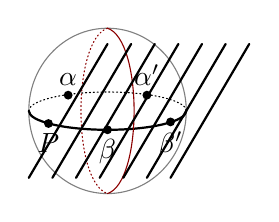
\begin{tikzpicture}[x=1cm,y=1cm,line cap=round,line join=round]\draw[gray] (0,0) ellipse (1 and 1.05);\draw[thick] (-1,0) arc[start angle=180,end angle=360,x radius=1,y radius=.24];\draw[densely dotted] (-1,0) arc[start angle=180,end angle=0,x radius=1,y radius=.24];\draw[red!55!black] (0,1.05) .. controls (.45,.9) and (.45,-.9) .. (0,-1.05);\draw[red!55!black,densely dotted] (0,1.05) .. controls (-.45,.9) and (-.45,-.9) .. (0,-1.05);\fill (-0.5,0.2) circle(1.6pt) node[above] {$\alpha$};\fill (0.5,0.2) circle(1.6pt) node[above] {$\alpha'$};\fill (-0.75,-0.16) circle(1.6pt) node[below] {$P$};\fill (0,-0.24) circle(1.6pt) node[below] {$\beta$};\fill (0.8,-0.14) circle(1.6pt) node[below] {$\beta'$};\draw[thick] (-1,-.85)--(0,.85);\draw[thick] (-0.7,-.85)--(0.30000000000000004,.85);\draw[thick] (-0.4,-.85)--(0.6,.85);\draw[thick] (-0.1,-.85)--(0.9,.85);\draw[thick] (0.2,-.85)--(1.2,.85);\draw[thick] (0.5,-.85)--(1.5,.85);\draw[thick] (0.8,-.85)--(1.8,.85);\end{tikzpicture}}}
\sbox{185}{\figure{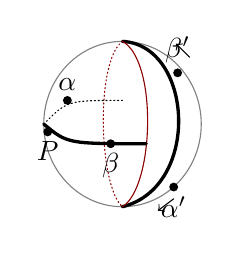
\begin{tikzpicture}[x=1cm,y=1cm,line cap=round,line join=round]\draw[gray] (0,0) ellipse (1 and 1.05);\draw[very thick] (0,1.05) .. controls (.9,1) and (1,-.8) .. (0,-1.05);\draw[red!55!black] (0,1.05) .. controls (.45,.8) and (.4,-.8) .. (0,-1.05);\draw[red!55!black,densely dotted] (0,1.05) .. controls (-.35,.8) and (-.3,-.8) .. (0,-1.05);\draw[very thick] (-1,0)..controls(-.7,-.25)..(.3,-.25);\draw[densely dotted] (-1,0)..controls(-.7,.3)..(0,.3);\fill (-0.7,0.3) circle(1.6pt) node[above] {$\alpha$};\fill (0.7,0.65) circle(1.6pt) node[above] {$\beta'$};\fill (-0.95,-0.1) circle(1.6pt) node[below] {$P$};\fill (-0.15,-0.25) circle(1.6pt) node[below] {$\beta$};\fill (0.65,-0.8) circle(1.6pt) node[below] {$\alpha'$};\draw[->] (.85,.85)--(.68,1.02);\draw[->] (.65,-.95)--(.45,-1.1);\end{tikzpicture}}}
\sbox{186}{\figure{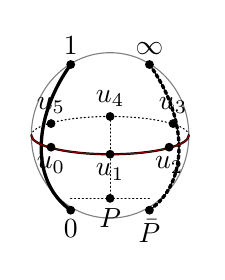
\begin{tikzpicture}[x=1cm,y=1cm,line cap=round,line join=round]\draw[gray] (0,0) ellipse (1 and 1.05);\draw[thick] (-1,0) arc[start angle=180,end angle=360,x radius=1,y radius=.24];\draw[densely dotted] (-1,0) arc[start angle=180,end angle=0,x radius=1,y radius=.24];\draw[very thick] (-.5,.9)..controls(-1,.2)and(-1,-.6)..(-.5,-.95);\draw[very thick,densely dotted] (.5,.9)..controls(1,.2)and(1,-.6)..(.5,-.95);\draw[red!55!black] (-1,0) arc[start angle=180,end angle=360,x radius=1,y radius=.24];\draw[densely dotted] (-.5,-.8)--(.5,-.8);\draw[densely dotted] (0,.24)--(0,-.8);\fill (-0.5,0.9) circle(1.6pt) node[above] {$1$};\fill (0.5,0.9) circle(1.6pt) node[above] {$\infty$};\fill (-0.5,-0.95) circle(1.6pt) node[below] {$0$};\fill (0.5,-0.95) circle(1.6pt) node[below] {$\bar P$};\fill (0,-0.8) circle(1.6pt) node[below] {$P$};\fill (-0.75,-0.15) circle(1.6pt) node[below] {$u_0$};\fill (0,-0.24) circle(1.6pt) node[below] {$u_1$};\fill (0.75,-0.15) circle(1.6pt) node[below] {$u_2$};\fill (0.8,0.15) circle(1.6pt) node[above] {$u_3$};\fill (0,0.24) circle(1.6pt) node[above] {$u_4$};\fill (-0.75,0.15) circle(1.6pt) node[above] {$u_5$};\end{tikzpicture}}}
\sbox{187}{\figure{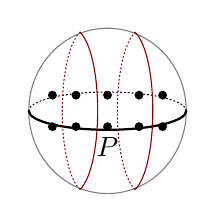
\begin{tikzpicture}[x=1cm,y=1cm,line cap=round,line join=round]\draw[gray] (0,0) ellipse (1 and 1.05);\draw[thick] (-1,0) arc[start angle=180,end angle=360,x radius=1,y radius=.24];\draw[densely dotted] (-1,0) arc[start angle=180,end angle=0,x radius=1,y radius=.24];\draw[red!55!black] (-0.35,1) .. controls (-0.04999999999999999,.7) and (-0.04999999999999999,-.7) .. (-0.35,-1);\draw[red!55!black,densely dotted] (-0.35,1) .. controls (-0.6499999999999999,.7) and (-0.6499999999999999,-.7) .. (-0.35,-1);\draw[red!55!black] (0.35,1) .. controls (0.6499999999999999,.7) and (0.6499999999999999,-.7) .. (0.35,-1);\draw[red!55!black,densely dotted] (0.35,1) .. controls (0.04999999999999999,.7) and (0.04999999999999999,-.7) .. (0.35,-1);\fill (-0.7,-0.2) circle(1.6pt);\fill (-0.7,0.2) circle(1.6pt);\fill (-0.4,-0.2) circle(1.6pt);\fill (-0.4,0.2) circle(1.6pt);\fill (0,-0.2) circle(1.6pt);\fill (0,0.2) circle(1.6pt);\fill (0.4,-0.2) circle(1.6pt);\fill (0.4,0.2) circle(1.6pt);\fill (0.7,-0.2) circle(1.6pt);\fill (0.7,0.2) circle(1.6pt);\node[below] at (0,-.22) {$P$};\end{tikzpicture}}}
\sbox{188}{\figure{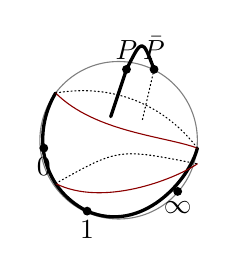
\begin{tikzpicture}[x=1cm,y=1cm,line cap=round,line join=round]\draw[gray] (0,0) circle(1);\draw[very thick] (-.8,.6)..controls(-1.1,.1)and(-1,-.6)..(-.4,-.9)..controls(.3,-1.2)and(.9,-.5)..(1,-.1);\draw[red!55!black] (-.8,.6)..controls(-.3,.1)and(.6,.05)..(1,-.1);\draw[densely dotted] (-.8,.6)..controls(.1,.75)and(.7,.3)..(1,-.1);\draw[red!55!black] (-.8,-.55)..controls(-.2,-.85)and(.7,-.5)..(1,-.3);\draw[densely dotted] (-.8,-.55)..controls(0,-.1)..(1,-.3);\draw[very thick] (-.1,.3)--(.1,.9)..controls(.3,1.3)..(.45,.9);\draw[densely dotted] (.45,.9)--(.3,.25);\fill (-0.95,-0.1) circle(1.6pt) node[below] {$0$};\fill (-0.4,-0.9) circle(1.6pt) node[below] {$1$};\fill (0.75,-0.65) circle(1.6pt) node[below] {$\infty$};\fill (0.1,0.9) circle(1.6pt) node[above] {$P$};\fill (0.45,0.9) circle(1.6pt) node[above] {$\bar P$};\end{tikzpicture}}}
\sbox{189}{\figure{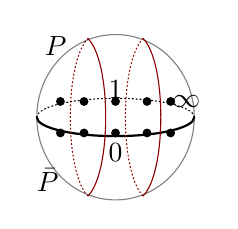
\begin{tikzpicture}[x=1cm,y=1cm,line cap=round,line join=round]\draw[gray] (0,0) ellipse (1 and 1.05);\draw[thick] (-1,0) arc[start angle=180,end angle=360,x radius=1,y radius=.24];\draw[densely dotted] (-1,0) arc[start angle=180,end angle=0,x radius=1,y radius=.24];\draw[red!55!black] (-0.35,1) .. controls (-0.04999999999999999,.7) and (-0.04999999999999999,-.7) .. (-0.35,-1);\draw[red!55!black,densely dotted] (-0.35,1) .. controls (-0.6499999999999999,.7) and (-0.6499999999999999,-.7) .. (-0.35,-1);\draw[red!55!black] (0.35,1) .. controls (0.6499999999999999,.7) and (0.6499999999999999,-.7) .. (0.35,-1);\draw[red!55!black,densely dotted] (0.35,1) .. controls (0.04999999999999999,.7) and (0.04999999999999999,-.7) .. (0.35,-1);\fill (-0.7,-0.2) circle(1.6pt);\fill (-0.7,0.2) circle(1.6pt);\fill (-0.4,-0.2) circle(1.6pt);\fill (-0.4,0.2) circle(1.6pt);\fill (0,-0.2) circle(1.6pt);\fill (0,0.2) circle(1.6pt);\fill (0.4,-0.2) circle(1.6pt);\fill (0.4,0.2) circle(1.6pt);\fill (0.7,-0.2) circle(1.6pt);\fill (0.7,0.2) circle(1.6pt);\node[left] at (-.5,.9) {$P$};\node[left] at (-.6,-.8) {$\bar P$};\node[right] at (.6,.2) {$\infty$};\node at (0,.35) {$1$};\node at (0,-.45) {$0$};\end{tikzpicture}}}
\sbox{190}{\figure{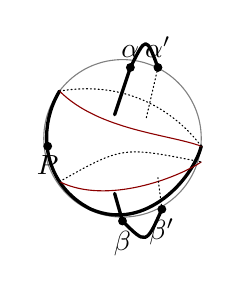
\begin{tikzpicture}[x=1cm,y=1cm,line cap=round,line join=round]\draw[gray] (0,0) circle(1);\draw[very thick] (-.8,.6)..controls(-1.1,.1)and(-1,-.6)..(-.4,-.9)..controls(.3,-1.2)and(.9,-.5)..(1,-.1);\draw[red!55!black] (-.8,.6)..controls(-.3,.1)and(.6,.05)..(1,-.1);\draw[densely dotted] (-.8,.6)..controls(.1,.75)and(.7,.3)..(1,-.1);\draw[red!55!black] (-.8,-.55)..controls(-.2,-.85)and(.7,-.5)..(1,-.3);\draw[densely dotted] (-.8,-.55)..controls(0,-.1)..(1,-.3);\draw[very thick] (-.1,.3)--(.1,.9)..controls(.3,1.3)..(.45,.9);\draw[densely dotted] (.45,.9)--(.3,.25);\draw[very thick] (-.1,-.7)--(0,-1.05)..controls(.3,-1.35)..(.5,-.9);\draw[densely dotted] (.5,-.9)--(.45,-.5);\fill (-0.95,-0.1) circle(1.6pt) node[below] {$P$};\fill (0.1,0.9) circle(1.6pt) node[above] {$\alpha$};\fill (0.45,0.9) circle(1.6pt) node[above] {$\alpha'$};\fill (0,-1.05) circle(1.6pt) node[below] {$\beta$};\fill (0.5,-0.9) circle(1.6pt) node[below] {$\beta'$};\end{tikzpicture}}}
\sbox{191}{\figure{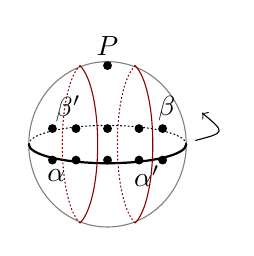
\begin{tikzpicture}[x=1cm,y=1cm,line cap=round,line join=round]\draw[gray] (0,0) ellipse (1 and 1.05);\draw[thick] (-1,0) arc[start angle=180,end angle=360,x radius=1,y radius=.24];\draw[densely dotted] (-1,0) arc[start angle=180,end angle=0,x radius=1,y radius=.24];\draw[red!55!black] (-0.35,1) .. controls (-0.04999999999999999,.7) and (-0.04999999999999999,-.7) .. (-0.35,-1);\draw[red!55!black,densely dotted] (-0.35,1) .. controls (-0.6499999999999999,.7) and (-0.6499999999999999,-.7) .. (-0.35,-1);\draw[red!55!black] (0.35,1) .. controls (0.6499999999999999,.7) and (0.6499999999999999,-.7) .. (0.35,-1);\draw[red!55!black,densely dotted] (0.35,1) .. controls (0.04999999999999999,.7) and (0.04999999999999999,-.7) .. (0.35,-1);\fill (-0.7,-0.2) circle(1.6pt);\fill (-0.7,0.2) circle(1.6pt);\fill (-0.4,-0.2) circle(1.6pt);\fill (-0.4,0.2) circle(1.6pt);\fill (0,-0.2) circle(1.6pt);\fill (0,0.2) circle(1.6pt);\fill (0.4,-0.2) circle(1.6pt);\fill (0.4,0.2) circle(1.6pt);\fill (0.7,-0.2) circle(1.6pt);\fill (0.7,0.2) circle(1.6pt);\fill (0,1) circle(1.6pt) node[above] {$P$};\node at (-.65,-.4) {$\alpha$};\node at (.5,-.4) {$\alpha^\prime$};\node at (-.5,.45) {$\beta^\prime$};\node at (.75,.45) {$\beta$};\draw[->] (1.12,.05)..controls(1.5,.15)..(1.2,.4);\end{tikzpicture}}}
\diagram{\begin{tikzcd}[ampersand replacement=\&,column sep=9em,row sep=10em]
\begin{gathered}\mathrm{I}_{10}\ (\text{pentagonale})\\
\figure{\usebox{180}}\\
\text{12 structures pentagonales sur }K\\
\{\sigma,\sigma^{-1}\}\in P_2\unsure{\mathrm{Circ}}(K)\\
G\simeq\mathbb D_5\\
\widetilde G\simeq\mathbb D_5\times\{1,\sigma\}\end{gathered}\&\begin{gathered}\mathrm I_6\ (\text{bitétraédrale})\\
\figure{\usebox{181}}\\
\text{20 structures }K=J\amalg\omega\\
\text{avec }\omega\xrightarrow{\sim}\underline\omega(J)\\
G\simeq\unsure{\mathfrak S}_J\simeq\unsure{\mathfrak S}_3\\
\widetilde G\simeq\unsure{\mathfrak S}_3\times\{1,\sigma\}\end{gathered} \arrow[r,"{3\quad f_{B,s}\quad2}","{(B\in\mathrm{Bit\acute et}(K),\ s\in\pi(B)=J)}"'] \& \begin{gathered}\mathrm I_4\ (\text{pyramidale})\\
\figure{\usebox{182}}\\
\text{30 structures carrés orientés}\\
K\simeq\{P\}\amalg I\\
I\ \text{structure carré \uline{orienté}}\ (Q,\omega)=\vec Q\\
I=\coprod_{\alpha\in\delta}\alpha\qquad\delta=\text{ens. des diagonales }\alpha\\
\omega\in\delta\wedge\bigwedge_{\alpha\in\delta}\alpha\\
G=\widetilde G=\mathbb Z/4\mathbb Z\end{gathered} \\
\begin{gathered}\mathrm{II}_2\ (\text{carré-triangle droit})\\
\figure{\usebox{183}}\\
\text{2 sommets-repères}\quad\deleted{\text{\unsure{repères}}}\\
\text{60 structures ``pentagone}\\
\text{avec sommet'' sur }K\\
\text{i.e. }K\simeq J\amalg\omega,\ \text{avec }\omega\hookrightarrow J\\
\text{i.e. }P\in J\text{ et }\omega\xrightarrow{\sim}\omega'=J\setminus\{P\}\\
G\simeq\mathbb Z/2\mathbb Z\\
\widetilde G\simeq\mathbb Z/2\mathbb Z\times\{1,\sigma\}\end{gathered} \arrow[u,"{1\quad\gamma_{\pi,s}\quad5}","{(\pi\in\mathrm{Pent}(K),\ s\in K)}"'] \arrow[r,"{1\quad\tau_{\pi,s}=\mathrm{tw}_{1/4}\quad1}"] \& \begin{gathered}\mathrm{II}'_2=\mathrm{Tw}_{1/4}\mathrm{II}_2\\
(\text{carré-triangle gauche})\\
\text{4 sommets}\ \deleted{\text{\unsure{repères}}}\\
\deleted{\figure{\usebox{184}}}\quad\figure{\usebox{185}}\\
\text{mêmes paramètres que }\mathrm{II}_2\\
G\simeq\mathbb Z/2\mathbb Z,\ \widetilde G\simeq\mathbb Z/2\mathbb Z\times\{1,\sigma\}\end{gathered} \arrow[u,"{\unsure{\gamma^1_{\pi,s}}\quad3}","{\text{comp. avec }\vec Q}"'] \arrow[ur,bend left=10,pos=.73,"{2\quad f_{\vec Q,\unsure{\omega},a}\quad4}","{(\vec Q\in\overrightarrow{\mathrm{Carr}}(K),\ a\in\unsure{\Lambda}(Q))}"'] \& \begin{gathered}\mathrm{II}_1\ (\text{tétraèdre-triangle})\\
\figure{\usebox{186}}\\
\text{6 sommets-repères}\\
\text{120 structures entièrement}\\
\text{épinglées,}\\
G=\deleted{\unsure{1}}=\{1\},\quad\widetilde G=\{1,\sigma\}\\
\left[\begin{gathered}K=J\amalg\varepsilon\quad\operatorname{card}J=3,\operatorname{card}\varepsilon=2\\\omega\in\underline\omega(J),\ r\in J\times\varepsilon\\\tau_r^0:\mathrm{II}_1(J,\varepsilon)\longrightarrow\mathrm{II}_1(u_\omega(r))\\\text{où }u_\omega=\omega\times(-1)\text{ sur }J\times\varepsilon\end{gathered}\right]\end{gathered} \arrow[ul,pos=.73,"{1\quad\gamma_r^0\quad6}","{\text{comp. avec }\vec Q;\ (\pi\in\mathrm{Pent}(K),s\in K)}"'] \arrow[loop right,"{\tau_r^0=\mathrm{tw}_{1/6}}"] \\
\begin{gathered}\mathrm{III}_2\ (\text{triple triangle droit})\\
\figure{\usebox{187}}\\
\text{2+2 sommets-repère}\\
\text{60 structures ``pentagone avec}\\
\text{sommet'' sur }K,\\
G=\mathbb Z/2\mathbb Z,\widetilde G\simeq\mathbb Z/2\mathbb Z\times\{1,\sigma\}\end{gathered} \arrow[u,"{2\quad\gamma_{\pi,\rho}\quad2}","{(\pi\in\mathrm{Pent}(K),\rho\in\mathrm{Rep}\,\pi)}"'] \arrow[r,"{2\quad\tau_{\pi,\rho}=\mathrm{tw}_{1/3}\quad1}"] \& \begin{gathered}\mathrm{III}_1\ (\text{triple triangle sem.-gauche})\\
\figure{\usebox{188}}\quad=\quad\figure{\usebox{189}}\\
\text{2+4 sommets-repère}\\
\text{120 structures épinglées}\\
G=1,\widetilde G=\{1,\sigma\}\end{gathered} \arrow[u,"{1\quad\gamma_r^1\quad2}"] \arrow[ur,"{3\quad\gamma_{\bar r}^1\quad3}","{(r\in\mathrm{Rep}(K))}"'] \arrow[ul,bend left=30,"{\gamma_r^2\quad2}"] \arrow[r,"{1\quad\tau_r^1\quad2}"] \& \begin{gathered}\mathrm{III}'_2\ (\text{triple triangle gauche})\\
\figure{\usebox{190}}\quad\simeq\quad\figure{\usebox{191}}\\
\text{4+4 sommets-repère}\\
\text{60 structures de carré orienté à}\\
\text{codiagonales, }K=\{P\}\amalg I,\\
I\ \text{muni d’une \inserted{str.} carré en codiagonales }\unsure{\delta}=\{\alpha,\beta,\alpha',\beta'\}\\
\text{i.e. d’un repère de }\unsure{\mathfrak X}(I)\\
G=\mathbb Z/2\mathbb Z\deleted{\unsure{*}},\quad\widetilde G\simeq\mathbb Z/2\mathbb Z\times\mathbb Z/2\mathbb Z\simeq\mathbb Z/2\mathbb Z\times\{1,\sigma\}\end{gathered} \arrow[uu,bend right=70,"{1\quad\gamma_r^{21}\quad2}"]
\end{tikzcd}}

\diagram{\[\begin{array}{lll}
\uline{\text{niveau }2}&\mathrm I_{10},\mathrm I_6,\mathrm I_4&12+20+30=62\\
\uline{\text{niveau }1}&\mathrm{II}_2,\mathrm{II}'_2,\mathrm{II}_1&60+60+120=240\\
\uline{\text{niveau }0}&\mathrm{III}_2,\mathrm{III}_1,\mathrm{III}'_2&60+120+60=240\\
&&\underline{542}
\end{array}\]}

(l’indice indique l’ordre de \(G=\operatorname{Aut}^{+}\) ; donc le nb de structures est \(120/i\))

\uline{NB} Sauf \(\mathrm I_4\), toutes ces structures sont ``réelles''.

\[\begin{array}{ll}
\pi\in\mathrm{Pent}(K),&B\in\mathrm{Bit\acute et}(K)\\
s\in K,&\vec Q\in\overrightarrow{\mathrm{Carr}}(K)\\
\rho\in\mathrm{Rep}(\pi);&r\in\mathrm{Rep}(K)
\end{array}\]
(\uline{NB} \(\{(\pi,\rho)\}\simeq\mathrm{Rep}(K)\)).
\unsure{\texttt{GUTS OUTPUT FOR PREDONT DELIVER AT 0000 - PREDONT.MODULEF5}}

\unsure{\texttt{GUTS OUTPUT FOR PREDONT DELIVER AT 0000 - PREDONT.MODULEF5}}

\unsure{\texttt{GUTS OUTPUT FOR PREDONT DELIVER AT 0000 - PREDONT.MODULEF5}}

\unsure{\texttt{GUTS OUTPUT FOR PREDONT DELIVER AT 0000 - PREDONT.MODULEF5}}

\unsure{\texttt{GUTS OUTPUT FOR PREDONT DELIVER AT 0000 - PREDONT.MODULEF5}}

\unsure{\texttt{GUTS OUTPUT FOR PREDONT DELIVER AT 0000 - PREDONT.MODULEF5}}

\unsure{\texttt{GUTS OUTPUT FOR PREDONT DELIVER AT 0000 - PREDONT.MODULEF5}}

\unsure{\texttt{GUTS OUTPUT FOR PREDONT DELIVER AT 0000 - PREDONT.MODULEF5}}

\unsure{\texttt{GUTS OUTPUT FOR PREDONT DELIVER AT 0000 - PREDONT.MODULEF5}}

\unsure{\texttt{GUTS OUTPUT FOR PREDONT DELIVER AT 0000 - PREDONT.MODULEF5}}

\unsure{\texttt{GUTS OUTPUT FOR PREDONT DELIVER AT 0000 - PREDONT.MODULEF5}}

\unsure{\texttt{GUTS OUTPUT FOR PREDONT DELIVER AT 0000 - PREDONT.MODULEF5}}

\unsure{\texttt{GUTS OUTPUT FOR PREDONT DELIVER AT 0000 - PREDONT.MODULEF5}}

\unsure{\texttt{GUTS OUTPUT FOR PREDONT DELIVER AT 0000 - PREDONT.MODULEF5}}

\unsure{\texttt{GUTS OUTPUT FOR PREDONT DELIVER AT 0000 - PREDONT.MODULEF5}}

\unsure{\texttt{GUTS OUTPUT FOR PREDONT DELIVER AT 0000 - PREDONT.MODULEF5}}

\unsure{\texttt{GUTS OUTPUT FOR PREDONT DELIVER AT 0000 - PREDONT.MODULEF5}}

\unsure{\texttt{GUTS OUTPUT FOR PREDONT DELIVER AT 0000 - PREDONT.MODULEF5}}

\unsure{\texttt{GUTS OUTPUT FOR PREDONT DELIVER AT 0000 - PREDONT.MODULEF5}}

\unsure{\texttt{GUTS OUTPUT FOR PREDONT DELIVER AT 0000 - PREDONT.MODULEF5}}

\unsure{\texttt{GUTS OUTPUT FOR PREDONT DELIVER AT 0000 - PREDONT.MODULEF5}}

\unsure{\texttt{GUTS OUTPUT FOR PREDONT DELIVER AT 0000 - PREDONT.MODULEF5}}

\unsure{\texttt{GUTS OUTPUT FOR PREDONT DELIVER AT 0000 - PREDONT.MODULEF5}}

\unsure{\texttt{GUTS OUTPUT FOR PREDONT DELIVER AT 0000 - PREDONT.MODULEF5}}

\unsure{\texttt{GUTS OUTPUT FOR PREDONT DELIVER AT 0000 - PREDONT.MODULEF5}}

\unsure{\texttt{GUTS OUTPUT FOR PREDONT DELIVER AT 0000 - PREDONT.MODULEF5}}

\unsure{\texttt{GUTS OUTPUT FOR PREDONT DELIVER AT 0000 - PREDONT.MODULEF5}}

\unsure{\texttt{GUTS OUTPUT FOR PREDONT DELIVER AT 0000 - PREDONT.MODULEF5}}
\mspage{30}
